\section{Performance-Evaluation}

Ein Audio-Plug-in läuft in einer Umgebung mit vielen anderen Komponenten, mit dem es CPU-Ressourcen teilt. Die Verarbeitung von Audiodaten muss innerhalb diskreten, von der Audio-Hardware gesteuerten, Zeitintervallen abgeschlossen werden. Typische Audio-Sampling-Frequenzen sind 44,1 kHz, 48 kHz, 88,2 kHz und 96 kHz. Mit 44,1 kHz als Beispiel bedeutet dies, dass die für eine einzelne Abtastung erforderlichen Berechnungen innerhalb von 0,023 ms durchgeführt werden müssen. Interrupts müssten von der Audio-Hardware in Abständen von 0.023ms getätigt werden, und dies würde das Betriebssystem der CPU überlasten. Stattdessen werden Anfragen für neue Audiodaten in Puffern gebündelt. Die Größe der Puffer ist ein Parameter, der vom Benutzer gesetzt werden kann. In der Regel beträgt er 512 Abtastungen, kann aber bis 16 Abtastungen klein sein.

Erhöht man die Puffergröße, steigt auch die Zeit, die die CPU hat, um die Audiodaten zu verarbeiten. Dies führt aber auch dazu, dass die Latenz des Systems steigt. Eine Puffergröße von 512 Abtastungen entspricht einer Latenzzeit von 11.60ms. Eine 16-Probenpuffer-Größe entspricht 0.36ms.

Braucht ein einzelnes Plug-in 1,0 ms, um seine Verarbeitung abzuschließen, dann wird es nicht rechtzeitig beendet, wenn die Puffergröße zu niedrig eingestellt ist. Wenn die Puffergröße gerade hoch genug ist, dann bleiben nicht genügend CPU-Ressourcen übrig für andere Plug-ins, ihre Berechnungen auszuführen.

\subsection{Synchrone Performance}

Dieses Projekt verteilt die Verarbeitung an externe SBC-Geräte. Es gibt jedoch keine Entlastung, wenn das Audio-Plug-in blockiert ist, während es für die Ergebnisse aus dem SBC-Gerät wartet. Da die externen SBC-Geräte langsamer sind als der Haupt-CPU, wird die Bearbeitungszeit sogar länger. Fügt man die Zeit hinzu, die zur Serialisierung und Deserialisierung des Datagramm-Pakets an jedem Ende benötigt wird, wird die Leistung sogar noch verschlechtert.

Abbildung~\ref{fig:local_vs_remote} zeigt das Problem genauer.

\begin{figure}[H]
    \centering
    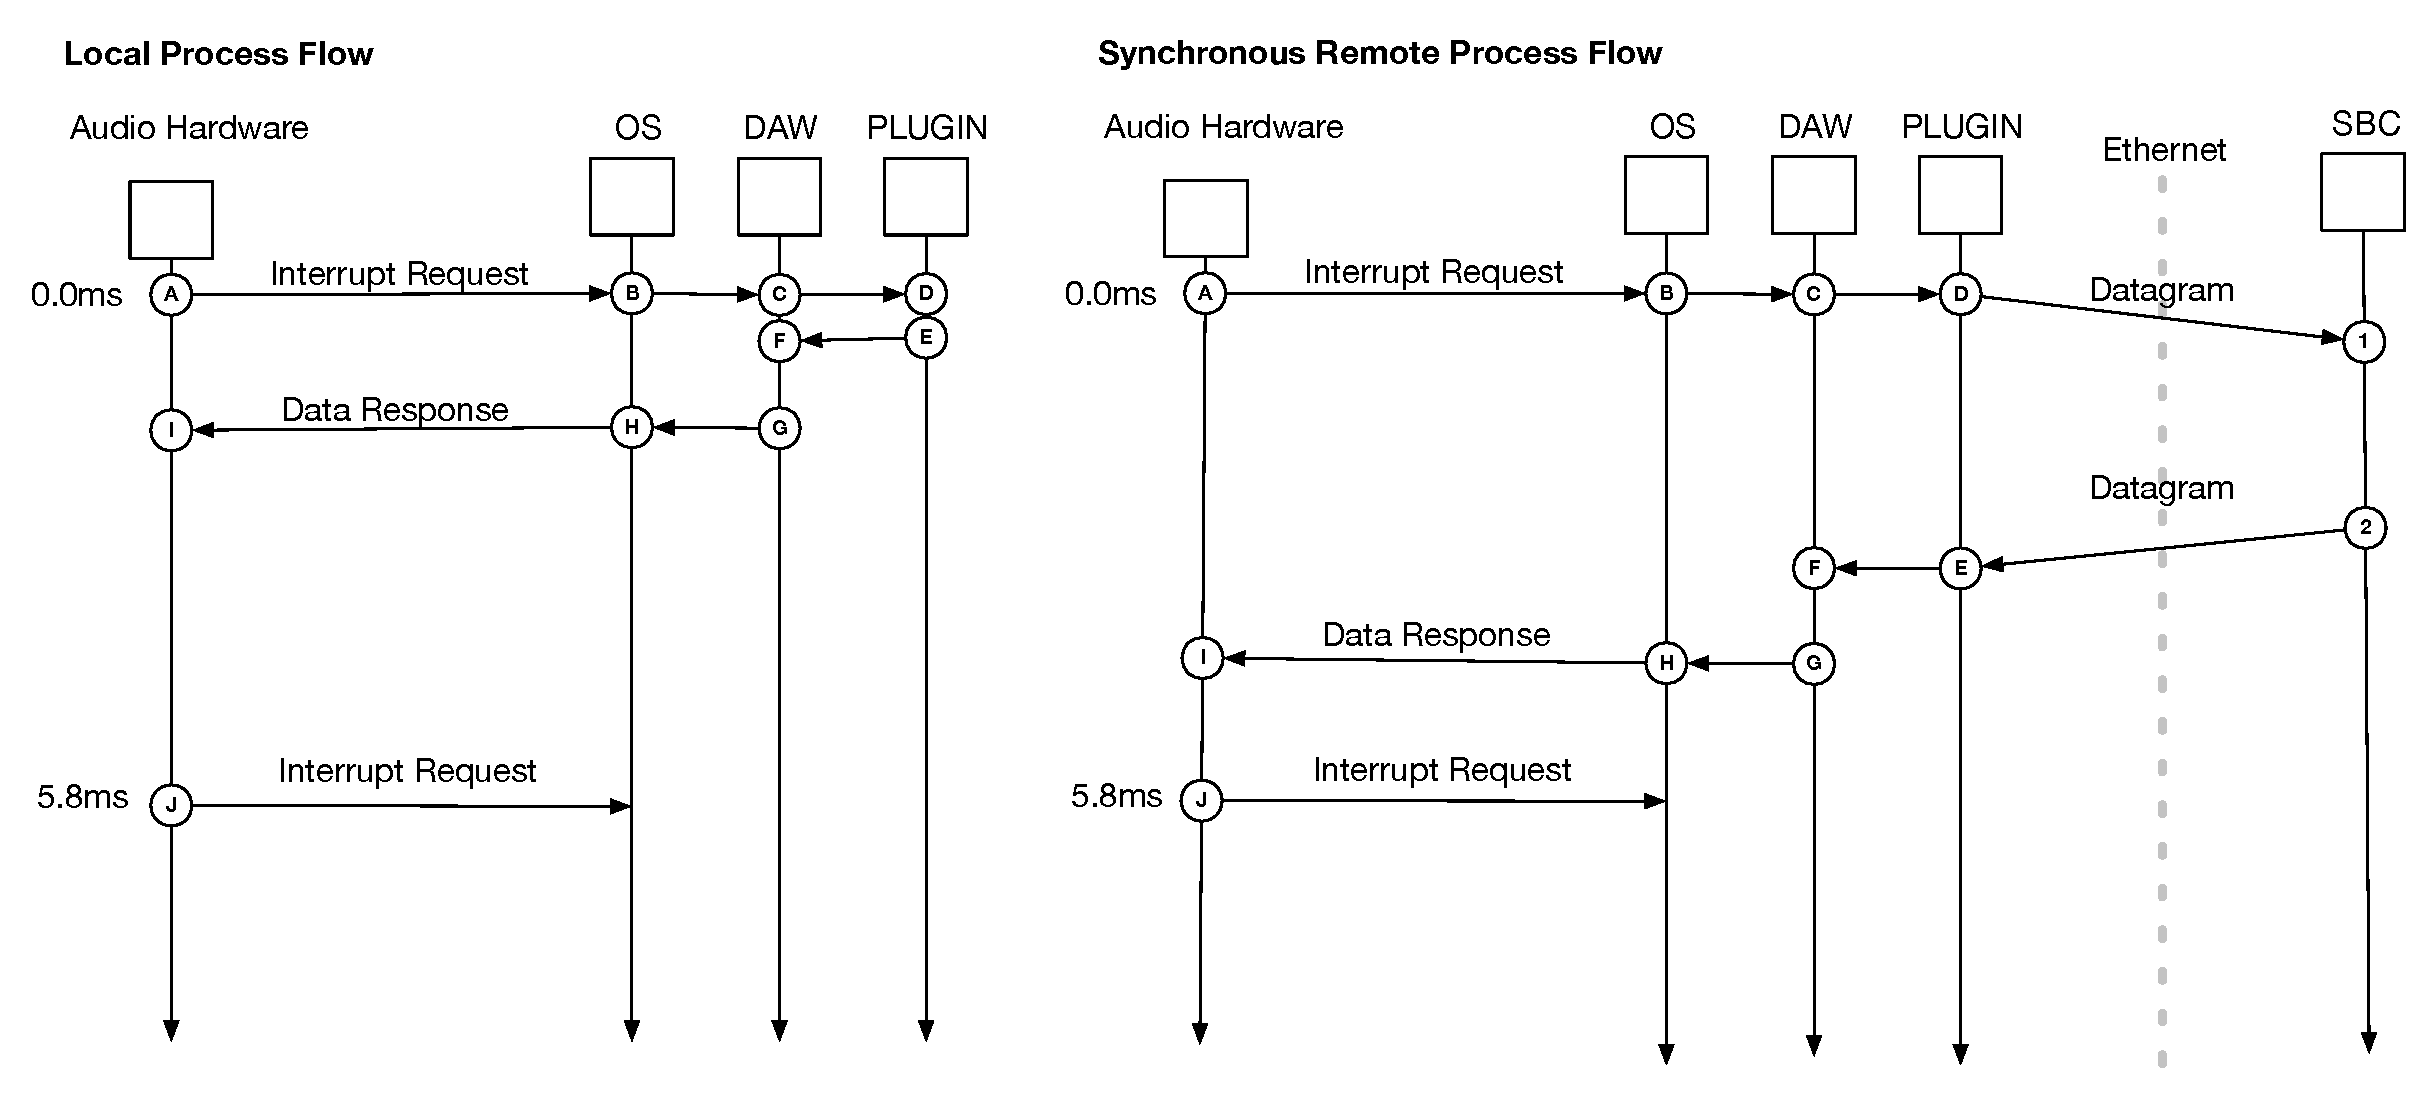
\includegraphics[width=\textwidth]{assets/conclusion/process_flow_compared.pdf}
    \caption{Lokale vs. externe synchrone Datenverarbeitung}
    \label{fig:local_vs_remote}
\end{figure}

Das Beispiel zeigt die Audio-Hardware-Abfragen an das Betriebssystem in Zeitintervallen von 5,8 ms getaktet. Dies entspricht einer Puffergröße von 256 Abtastwerten. Das Zeitintervall zwischen den Zuständen D und E repräsentiert die Zeit, die ein Plug-in braucht, um einen Puffer von 256 Proben zu verarbeiten. Die DAW-Anwendung führt andere notwendige Audio-Verarbeitungsfunktionen in dem Intervall zwischen F und G durch. Nach Zuständen G und H sind DAW-Anwendung und Betriebssystem wieder in der Lage, andere Dinge zu tun, wie z.B. die GUI zu aktualisieren.

Mit der synchronen verteilten Verarbeitung wird der Zustand E blockiert bis Zustände 1 und 2 abgeschlossen sind. Ist diese Zeit signifikant, hindert dies DAW-Anwendung und Betriebssystem daran, andere wichtige Aufgaben durchzuführen.

\begin{table}[H]
\begin{center}
\begin{tabular}{ |p{1.4cm}||p{1.5cm}|p{1.7cm}|p{1.7cm}|p{1.6cm}|p{1.4cm}|  }
 \hline
 puffergrösse    & pufferzeit (ms)    & rtTime (ms)   & pTime (ms)    & tTime (ms) & \% von pufferzeit\\
 \hline
 64             & 1.451247      & 0.574672          & 0.015857          & 0.558815      & 39.59 \\
 96             & 2.176870      & 0.575419          & 0.015851          & 0.559568      & 26.43 \\
 128            & 2.902494      & 0.59001           & 0.016519          & 0.573491      & 20.32 \\
 192            & 4.353741      & 0.67902           & 0.019013          & 0.660007      & 15.59 \\
 256            & 5.804988      & 0.707267          & 0.020352          & 0.686915      & 12.18 \\
 512            & 11.60997      & 0.707905          & 0.026348          & 0.681557      & 6.097 \\
 \hline
\end{tabular}
\end{center}
\caption{Measured Times for Synchronous Processing}
\label{tab:latency_comp}
\end{table}

Tabelle~\ref{tab:latency_comp} zeigt die gemessenen Zeiten für verschiedene Puffergrößen in der synchronen Ausführung, in der keine tatsächliche Audioverarbeitung stattfindet. Nur die Vorbereitungs- und Transport-Zeiten werden berücksichtigt. Ein Audiosystem, das  mit einer Puffergröße von 64 Proben läuft, hat 1.451ms, um alle Aufgaben zu erledigen. „rtTime“ ist die gemessene Gesamtumlaufzeit. Dies entspricht der Zeit zwischen den Zuständen D und E des synchronen Verfahrens in Abbildung~\ref{fig:local_vs_remote}. „pTime“ ist das Zeitintervall zwischen den Zuständen 1 und 2 auf dem SBC-Gerät, der Zeitaufwand für die Verarbeitung der Daten. In diesem Fall gab es keine Verarbeitung, so ist dies nur der für die Deserialisierung und Serialisierung der Datagramme zu Audio- und MIDI-Daten benötigte Zeitaufwand. „tTime“ ist die „pTime“, subtrahiert von der „rtTime”, welche dem Verpackungsaufwand entspricht, um Daten zu senden und zu empfangen.

Die letzte Spalte, "\% von pufferzeit”, zeigt, wie viel Zeit insgesamt als prozentualer Anteil verbraucht wurde. Bei einer Puffergröße von 64 Abtastungen wird 39.59 \% Prozent der Gesamtzeit für ein einziges Plug-in verbraucht. Es bleibt nicht viel Zeit übrig für andere Prozesse auf der CPU. Für eine Puffergröße von 512 Samples ist der Prozentsatz des Grenzwertes viel niedriger. Dafür ist aber die Gesamtsystemlatenz geringfügig höher als die maximal angestrebten 10ms. Durch die synchrone Implementierung wird die Verarbeitungslast der CPU überhaupt nicht verringert.


\subsection{Asynchrone Performance}

Anstatt auf eine Antwort von dem SBC zu warten wie bei der obigen synchronen Methode, prüft die asynchrone Methode zuerst, ob Daten vorhanden sind. Wenn ja,   diese sofort zurückgeben, wenn nicht, leere Daten zurückgeben. Die erste Anfrage für Audiodaten würde leere Daten zurückgeben, aber bis der zweite Puffer angefordert wird, könnte die erste Antwort bereits vom SBC-Gerät zurückgekommen sein. In beiden Fällen ist die einzige Zeit, die das Audio-Plug-in selbst verbraucht, nur für die Serialisierung, Deserialisierung und denTransport der Daten. Das sind die Zeitabstände zwischen den Zuständen D und E sowie M und N, dargestellt in Abbildung~\ref{fig:async_remote}.

\begin{figure}[H]
    \centering
    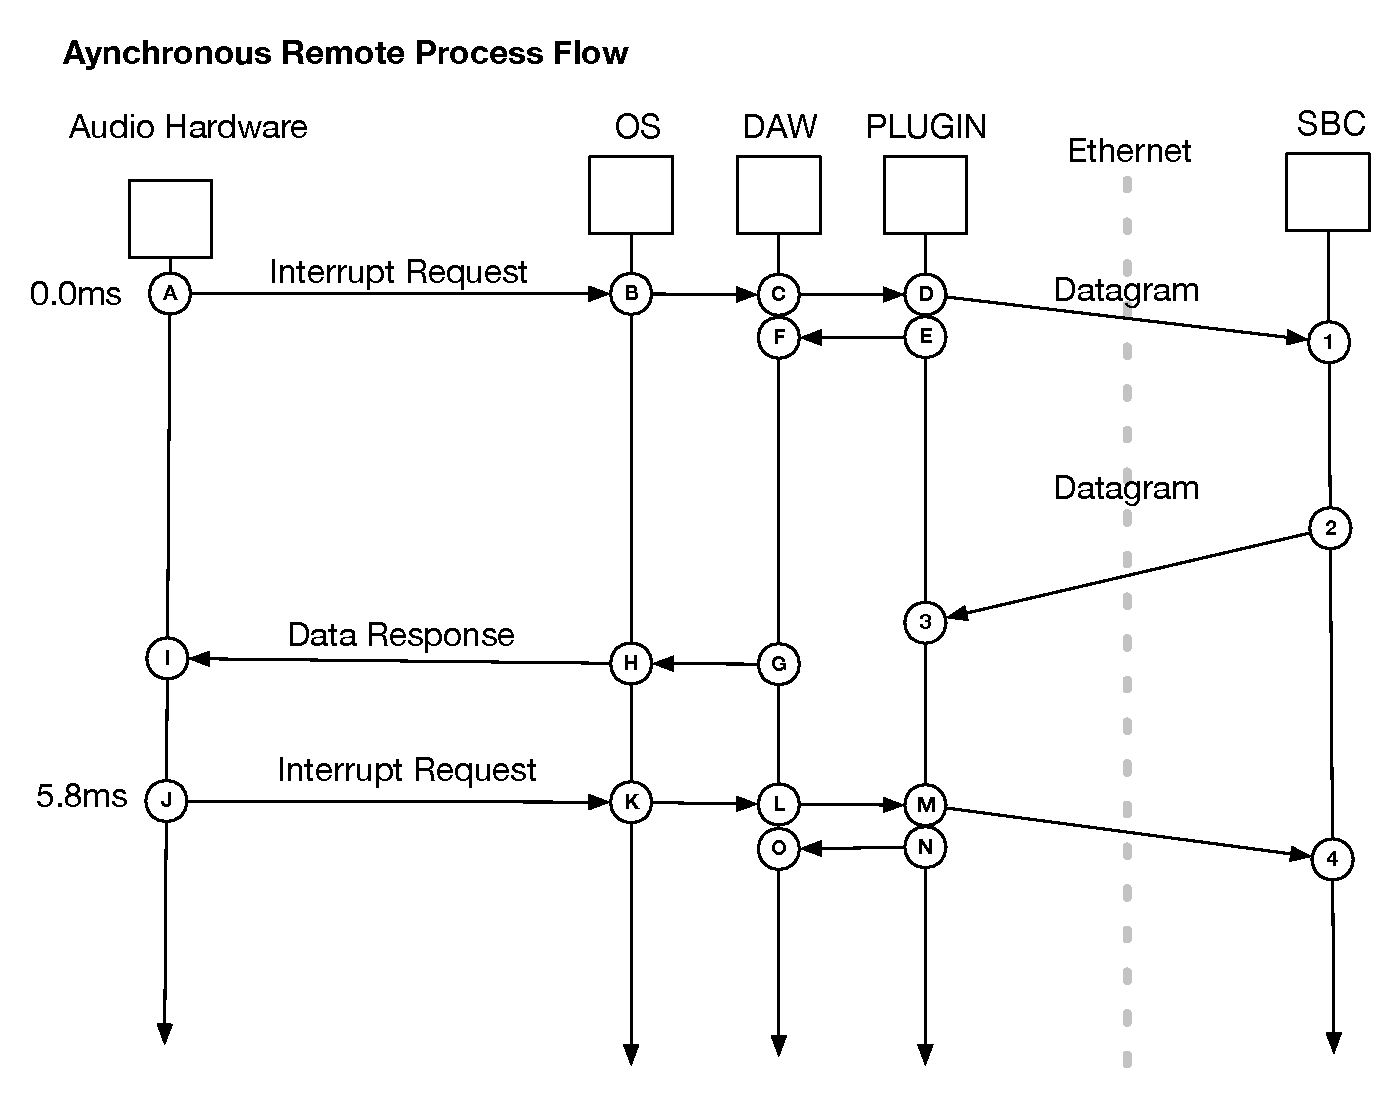
\includegraphics[width=\textwidth]{assets/conclusion/async_flow.pdf}
    \caption{Lokale vs. externe synchrone Datenverarbeitung}
    \label{fig:async_remote}
\end{figure}

Bis der zweite Zyklus beginnt (J in Abbildung~\ref{fig:async_remote}), sind die verarbeiteten Daten aus dem ersten Zyklus zurückgekehrt. Die Zeit zwischen den Ereignissen M und N ist nicht mehr proportional zum für die Datenverarbeitung tatsächlich benötigten Zeitaufwand, sondern lediglich zu der Zeit, die für das Senden und Empfangen der Daten benötigt wird. Tabelle B zeigt die gemessenen Zeiten.

\begin{table}[H]
\begin{center}
\begin{tabular}{ |p{1.4cm}||p{1.5cm}|p{1.7cm}|p{1.7cm}|p{1.6cm}|p{1.4cm}|  }
 \hline
 puffergrösse    & pufferzeit (ms)    & rtTime (ms)   & pTime (ms)    & tTime (ms) & \% von pufferzeit\\
 \hline
 64             & 1.451247      & 0.031683          & 0.015633          & 0.016050      & 2.18 \\
 96             & 2.176870      & 0.046585          & 0.016076          & 0.030509      & 2.14 \\
 128            & 2.902494      & 0.034745          & 0.016712          & 0.018032      & 1.19 \\
 192            & 4.353741      & 0.052279          & 0.018800          & 0.033478      & 1.20 \\
 256            & 5.804988      & 0.065752          & 0.019646          & 0.046105      & 1.13 \\
 512            & 11.60997      & 0.062939          & 0.019708          & 0.043230      & 0.54 \\
 \hline
\end{tabular}
\end{center}
\caption{Für asynchrone Datenverarbeitung gemessene Zeiten}
\label{tab:latency_async}
\end{table}



In der obigen Tabelle entspricht „rtTime” nicht mehr der tatsächlichen Gesamtverarbeitungszeit. Da die Daten zum Zeitpunkt des Interrupts bereits vorhanden sind, kann das Plug-in diese Daten sofort zurückzugeben. Dies geht auf Kosten der Latenzzeit, welche jetzt genau einem Interrupt-Zyklus entspricht. Der Benutzer kann die Puffergröße des Audiosystems so einstellen, dass dies weit unter der 10ms-Grenze ist, ohne dass mehr als 1,2 \% der Bearbeitungszeit verwendet wird.

Das asynchrone Verfahren bringt einen echten Nutzen für die verteilte Verarbeitung in Bezug auf die Belastung der CPU. Der Preis ist jedoch eine Erhöhung der Latenzzeit des Plug-ins. Verarbeitete Audiodaten sind immer um einen Puffer-Zyklus verzögert. Ein weiterer Nachteil ist, dass, wenn mehrere dezentrale Prozessoren in einer Reihe verkettet sind, wie dies in der Demo-Anwendung der Fall ist, die Latenzzeit dann kumulativ ist. Dies resultiert in einer Gesamtlatenz, d.h. der mit der Anzahl der Prozessoren im Plug-in multiplizierten Gesamtwert-Zeit.

\subsection{Mögliche Optimierungen}

Es gibt zwei Bereiche, in denen unnötige Operationen durchgeführt werden, die optimiert werden könnten. Der erste ist die Serialisierung und Deserialisierung von Daten, wenn sie vom SBC-Gerät zurückgegeben werden. Sind im Plug-in mehrere Prozesse nacheinander verkettet, wird die zurückgesandte DiauproMessage zwischen jedem Prozessschritt unnötig deserialisiert und reserialisiert. Dies wäre eine relativ einfach zu implementierende Optimierung.

Die zweite Optimierung ist ähnlich, aber komplizierter zu implementieren. In einer Kette nacheinander geschalteter Prozessen müssten die Daten nicht nach jedem Schritt an das Master-Plug-in zurückgeschickt werden, sondern direkt an den nächsten Knoten. Wenn sich der nächste Knoten auf dem gleichen SBC-Gerät befindet, wird ein zusätzlicher Schritt über Ethernet eingespart. Außerdem könnten auch die Serialisierungsschritte zwischen den Knoten übersprungen werden, wenn die Knoten ihre Berechnungen direkt auf den Daten in dem DiauproMessage ausführen. Hierzu müsste die DiauproMessage erweitert werden, um Routing-Informationen zu erfassen, so dass jeder Rechenknoten weiß, wohin die Daten als nächstes geschickt werden müssen.

Obwohl komplexer, hat die zweite Optimierung den zusätzlichen Vorteil, dass die Latenzzeit sich nicht um ein Vielfaches der vollen Zykluszeit zwischen Interrupt-Aufrufe multipliziert. Die endgültigen Daten könnten nach einem einzigen Interrupt-Zyklus zurückgegeben werden.

\section{Zusammenfassung}

Die asynchrone Umsetzung bietet deutliches Potenzial. Die Latenz scheint der von kommerziellen DSP-basierten Systemen zu entsprechen\cite{UAD2-review}. Dies ist interessant, da es zeigt, dass der DSP und die SBC-basierten Systeme die gleichen Limitierungen teilen, die nicht einfach durch einfaches Hinzufügen von mehr Rechenleistung überwunden werden. Die wirkliche Barriere besteht im schnellstmöglichen Datentransport, ohne dabei den Audio-Thread zu blockieren. Ob der Audio-Thread 10 \% oder 30 \% der Zeit blockiert wird, ist irrelevant. Entscheidet man sich für ein asynchrones Verfahren, das einen vollen Zyklus des Audiog-Threads überspringt, besteht keine Notwendigkeit, ihn zu blockieren. Der Unterschied in der Bandbreite zwischen Thunderbolt-, PCIe- oder Gigabit-Ethernet-Schnittstellen hat nur Auswirkungen auf die mögliche Anzahl laufender Plug-ins, aber nicht deren Latenz.

Dies ist ermutigend, insbesondere unter Berücksichtigung der Erweiterbarkeit des SBC-basiertes Systems, und der Kompatibilität der Codebasis. Zwei entscheidende Vorteile, die das SBC-System gegenüber DSP-basierten Systemen hat.
